\chapter{Modular Grasping Pipeline Architecture}
\label{cap4:modular_grasping_architecture}

Nowadays, since a completely generic solution, independently from previous knowledge of object shape, gripper design, and sensing type, is not an available option, there is a gap between real application, research development and scientific evaluation. Thus, creating a re-configurable grasping framework integrating the best of all methodologies could transfer this to a practical robotic grasping task which is the main contribution of the present thesis.

The core of the developed grasping planning architecture pipeline is divided into two parts: the grasping synthesis and the grasping selection (Figure~\ref{fig:grasping_framework_code}). In summary, the grasping synthesis is a system architecture responsible for generating all the grasping poses. It creates a set of  hypothetical grasping candidates in an offline step, i.e., it runs outside the robot system in a setup phase. The generated data is then uploaded to the robot system to be used during the grasping selection step. This architecture is responsible for choosing the best grasping candidate following a set of heuristics and priorities. It is a task-oriented procedure that analyses the environment and the run-time constraints of the task. The following sections provide a detailed description of the procedure.

\begin{figure}[h!]
\begin{tcolorbox}
% \centerline{\includegraphics[trim={7cm 8cm 7cm 9cm},clip,width=1\linewidth,angle=0]{Cap2/Figuras/friction_contact.pdf}}
\centerline{\includegraphics[trim={0cm 15cm 0cm 0cm},clip,width=0.95\linewidth,angle=0]{Cap4/Figuras/grasping_framework.pdf}}
\end{tcolorbox}
\caption{Proposed modular grasping architecture.}
\label{fig:grasping_framework_code}
\end{figure}

\section{Grasping Synthesis}
\label{cap4:modular_grasping_architecture:sec:grasping_synthesis}

The ``Grasping Synthesis'' is a set of tools responsible, in a pipeline fashion, for generating and handling the grasping poses dataset. This pipeline is an offline step, i.e., it runs outside the robot system in a setup phase. The dataset is created as a set of hypothetical grasping pose candidates which are hierarchically structured in a YAML file format. The proposed dataset standard is detailed discussed in Section~\ref{cap4:modular_grasping_architecture:sec:grasping_dataset}.

Currently three main components constitutes the grasping synthesis: the ``GraspIt!'' Interface (Section~\ref{cap4:modular_grasping_architecture:sec:grasping_synthesis:subsec:graspit}), the Mimic Grasping Module (Section~\ref{cap4:modular_grasping_architecture:sec:grasping_synthesis:subsec:mimic_grasping}) and the Post-Processor Pipeline (Section~\ref{cap4:modular_grasping_architecture:sec:grasping_synthesis:subsec:post_processor}). 

\subsection{Grasping Dataset Standard}
\label{cap4:modular_grasping_architecture:sec:grasping_dataset}

A grasping candidate, also referred as candidate, is defined by its pose over an object geometry. Besides this fundamental characteristic, others should be defined according to gripper in usage. Therefore, a structured grasping candidate dataset is proposed. This is a standard which allows new increments according to new future grippers addition.

The candidates are specified by an YAML descriptor (Snippet \ref{code:candidates_dataset}) and they are sequentially located in a YAML configuration file. %This dataset file can be loaded in the ROS parameter server afterwards. 

%\begin{minipage}{1\textwidth}
\begin{snippet}[h!]
	\centering
	\resizebox{0.75\textwidth}{!}{%	
	\begin{tcolorbox}
	\lstinputlisting[%caption= The candidate dataset descriptor example.,
	                  abovecaptionskip=3pt,
	                  captionpos=b,
	                  style=yaml,
	                  linerange={0-18},
	                  firstnumber=25,
	                  %label=code:candidates_dataset
	                  ]
	                  {Cap4/codes/candidates_dataset.yaml}
	\end{tcolorbox}
	}
	\caption{The candidate dataset descriptor example.}
	\label{code:candidates_dataset}
\end{snippet}
%\end{minipage}

The candidates are unique for gripper-object, therefore there exists one datatset per active pair, and they are named as ``candidate$\_$id'', where id is a integer that defines the order into datatset. 

Since the dataset standard is created focused on being applied to a modular grasping pipeline, which allows the integration of different methodologies, the first parameter, ``method/type'' is an integer that defines which synthesis method builds the candidate. Based on the configurable premiss, the supported gripper is defined by an integer code by ``gripper/type'' parameter followed by the ``gripper/parameters'' array. This dynamic size array is related to more complex grippers such as the adaptive RobotiQ models~\cite{robotiq_grippers} that grant more joints control. The ``gripper/type'' parameter define how to read this array, e.g for gripper type 0 (RobotiQ 2f84) and 1 (RobotiQ 2f140) the sequence is: force [N], velocity[m/s], pre-grasp-width [m], grasp-width [m], grasp-release-width [m], grasping model. On the other hand, grippers such as HGPC16A (Figure~\ref{fig:mimic_grippers_supported}) have an empty array since the control is performed only by the ON/OFF state. Any new model added to architecture should have this array described and defined. The ``gripper/DOFs'' is also a dynamic size array with fingers' joints \acp{DOF} value. Since the grasping candidate could be defined by the \textit{eingengrasp} (Section~\ref{sec:sim_ann}) or by the individual finger joint state, the ``method/type" defines how to extract this information from the array. Another important parameter to define this array is the ``gripper/type''. 

The position is given in meters followed by the orientation in quaternion w.r.t. ``parent$\_$frame$\_$id'' reference frame which if it is not declared, is considered the object reference;


%The others descriptor parameters are defined below:

%\begin{itemize_jp}
%    \item \textbf{method/type:} an integer that defines which synthesis method build the candidate. %Supported values in current thesis are: 0$\_$MANUAL, 1-SANN$\_$MULTIFINGERED, 2-SANN$\_$SUCTION. 3-MIMIC$\_$GRASPING;
%    \item \textbf{gripper/type:} an integer that defines the gripper type. %Supported values in current thesis are: 0-ROBOTIQ$\_$2F$\_$85, 1-ROBOTIQ$\_$2F$\_$140, 2-ROBOTIQ$\_$3F, 3-SUCTION, 4-FESTO$\_$2F$\_$HGPC$\_$16$\_$A, 5-SCHMALZ$\_$SINGLE$\_$RECT$\_$SUCTION;
%    \item \textbf{gripper/parameters:} a dynamic size array with specific gripper's parameters. Typically these parameters are related to more complex grippers such as Robotiq models~\cite{robotiq_grippers}. The ``gripper/type'' parameter define how to read this array, e.g for gripper type 0 (robotiq 2f84) and 1 (robotiq 2f140) the sequence is: force [N], velocity[m/s], pre-grasp-width [m], grasp-width [m], grasp-release-width [m], grasping model. On the other hand, grippers such as HGPC16A (Figure~\ref{fig:mimic_grippers_supported}) have a empty array since the control is performed only by ON/OFF state. Any new model added into architecture should have this array described and defined;
%    \item \textbf{gripper/DOFs:} a dynamic size array with fingers' joints \acp{DOF} value. Since the grasping candidate could be defined by the eingengrasp (Section~\ref{ap:sim_ann}) or by the individual finger joint state, the ``method/type" defines how to extract this information from the array. Another important parameter to define this array is the ``gripper/type''; 
%    \item \textbf{parent$\_$frame$\_$id:} reference frame in which the candidate is defined. If it is not declared, it is considered the object reference;
%    \item \textbf{position:} position w.r.t. parent frame id, in meters.
%    \item \textbf{orientation:} orientation w.r.t. parent frame id, in quaternion.
%\end{itemize_jp}

\subsection{``GraspIt" Interface}
\label{cap4:modular_grasping_architecture:sec:grasping_synthesis:subsec:graspit}

The ``GraspIt!" interface is responsible to generate grasping candidates based on CAD modelling by using the ``GraspIt!" API and simulator (Figure~\ref{fig:graspit_manual_feeder_workflow}), in association with \ac{ROS} framework. This simulator was first proposed by~\cite{miller2004graspit} and is widely used in academic community to multi-fingered grasping analysis (Section~\ref{sec:multifingered_grasping}) using CAD interaction in virtual environment. The grippers are structured in XML format (besides the 3D model, the \ac{ICR} and the \textit{eigengrasps}, Section~\ref{sec:sim_ann}, are also defined). The objects are included by using a Polygon File Format (extension ``.ply'').

\begin{figure}[h!]
	\resizebox{1\textwidth}{!}{%
		\begin{tcolorbox}
			\centerline{\includegraphics[trim={0cm 0cm 1cm 0cm},clip,width=1\linewidth,angle=0]{Cap4/Figuras/graspit_manual_support.pdf}}
		\end{tcolorbox}
		\caption{``GraspIt!" interface and the implemented manual feeder.}
		\label{fig:graspit_manual_feeder_workflow}
	}%end resize box
\end{figure}

The Figure~\ref{fig:grasping_graspit_module_workflow} presents the ``GraspIt" interface pipeline workflow.

\begin{figure}[h!]
\resizebox{1\textwidth}{!}{%
\begin{tcolorbox}
\centerline{\includegraphics[trim={0.5cm 3cm 17cm 0cm},clip,width=1\linewidth,angle=0]{Cap4/Figuras/flowchart_graspit_module.pdf}}
\end{tcolorbox}
\caption{``GraspIt!" interface pipeline workflow. }
\label{fig:grasping_graspit_module_workflow}
}%end resize box
\end{figure}

The implemented methods are discussed into Sections~\ref{cap4:modular_grasping_architecture:sec:grasping_synthesis:subsec:graspit:subsubsec:manual} and~\ref{cap4:modular_grasping_architecture:sec:grasping_synthesis:subsec:graspit:subsubsec:sann}. The interface is based on C++ polymorphic classes which allows new heuristics design and also incorporate new future ``GraspIt!" functionalities. 

\subsubsection{Manual Feeder}
\label{cap4:modular_grasping_architecture:sec:grasping_synthesis:subsec:graspit:subsubsec:manual}

The manual feeder allows the user to define grasping postures by interacting with ``GraspIt!" 3D environment, Figure~\ref{fig:graspit_manual_feeder_workflow}. This feeder automatic call and configure the ``GraspIt!" virtual interface. It also call a menu, which allows the operator to store, delete, manipulate the gripper and generate the grasping dataset based on the thesis' proposed standard (Section~\ref{cap4:modular_grasping_architecture:sec:grasping_dataset}). The YAML descriptor is defined in Snippet~\ref{code:manual_feeder}. %and its parameters is presented below:

%\begin{minipage}{1\textwidth}
\begin{snippet}[h!]
	\centering
	\resizebox{0.75\textwidth}{!}{%
	\begin{tcolorbox}
	 \lstinputlisting[%caption= The ``GraspIt!" manual descriptor example.,
	                  abovecaptionskip=3pt,
	                  captionpos=b,
	                  style=yaml,
	                  linerange={0-14},
	                  firstnumber=25,
	                  %label=code:manual_feeder
	                  ]
	                  {Cap4/codes/manual_feeder.yaml}
	\end{tcolorbox}
	}
	\caption{The ``GraspIt!" manual descriptor example.}
	\label{code:manual_feeder}
\end{snippet}
%\end{minipage}

%\begin{itemize_jp}
%    \item \textbf{path/gripper$\_$models$\_$file$\_$path:} path to locate the gripper XML model;
%    \item \textbf{path/object$\_$models$\_$file$\_$path:} path to locate the object ``.ply" model;
%    \item \textbf{gripper$\_$file$\_$name:} gripper XML file name;
%    \item \textbf{object$\_$file$\_$name:} object polygon file format name;
%    \item \textbf{config$\_$grasps$\_$parameters/gripper$\_$id:} gripper ID code;
%    %\item \textbf{config$\_$grasps$\_$parameters/grasp$\_$model: } 
%    %\item \textbf{config$\_$grasps$\_$parameters/velocity: } approach velocity. 
%    %\item \textbf{config$\_$grasps$\_$parameters/force: }
%    \item \textbf{config$\_$grasps$\_$parameters/approach$\_$width$\_$multiplier:} the multiplier to define the grasping width in approach procedure. This value is applied over the grasping candidate width;
%    \item \textbf{config$\_$grasps$\_$parameters/release$\_$width$\_$multiplier:} the multiplier to define the grasping width in release procedure. This value is applied over the grasping candidate width;
%    \item \textbf{config$\_$grasps$\_$parameters/min$\_$width$\_$threshold:} minimum width to consider in grasping procedure. Some grippers have flexible finger that need to be considered.
%\end{itemize_jp}

The gripper model path and name are defined in ``$path/gripper$\_$models$\_$file$\_$path$'' and ``$gripper$\_$file$\_$name$'', respectively. It should respect the ``GraspIt!'' XML description standard with its \ac{ICP}, \textit{eigengrasp} and Denavit-Hatenberg definitions. Focused on pipeline configurability, the gripper code ID is defined in ``$config$\_$grasps$\_$parameters/gripper$\_$id$'' and it is mapped according to the pipeline implementation. Other custom parameters are the ``$approach$\_$width$\_$multiplier$'' and ``$release$\_$width$\_$multiplier$'' which are multiplication factors to define the grasping width in the approach and release procedure. These values are applied over the grasping candidate width and it is important to avoid possible collision between the fingers during the grasping approaching and placing approaching movement.  The ``$config$\_$grasps$\_$parameters/min$\_$width$\_$threshold$'' is the minimum width to consider in grasping procedure. Some grippers have a flexible finger that needs to be considered.
In the end, the polygon file format of the object model should be defined by ``$path/object$\_$models$\_$file$\_$path$'' and ``$object$\_$file$\_$name$''.


\subsubsection{\acl{SANN} based Feeder}
\label{cap4:modular_grasping_architecture:sec:grasping_synthesis:subsec:graspit:subsubsec:sann}

The ``Graspit!" has support to grasping automatic generation by using the Very Fast \acl{SANN} optimisation algorithm. For a detailed explanation referrer to Section~\ref{sec:sim_ann}. This functionality is also incorporated into the core pipeline by the YAML descriptor presented in Snippet~\ref{code:multifingered_sann}. Besides the multi-fingered approach (Section~\ref{sec:multifingered_grasping}), a descriptor to suction grippers is designed considering that good suction grasping is directly related to well define contact point Snippet~\ref{code:suction_sann}.

%\begin{minipage}{1\textwidth}
\begin{snippet}[h!]
\centering
\resizebox{0.75\textwidth}{!}{%
\begin{tcolorbox}
 \lstinputlisting[
                  %caption= The ``GraspIt!" multi-finger\ac{SANN} YAML descriptor example.,
                  abovecaptionskip=3pt,
                  captionpos=b,
                  style=yaml,
                  linerange={0-34},
                  firstnumber=25,
                  %label=code:multifingered_sann
                  ]
                  {Cap4/codes/multifingered_sann_feeder.yaml}
\end{tcolorbox}
}
\caption{The ``GraspIt!" multi-finger \ac{SANN} YAML descriptor example.}
\label{code:multifingered_sann}
\end{snippet}
%\end{minipage}


%\begin{minipage}{1\textwidth}
\begin{snippet}[h!]
\centering
\resizebox{0.75\textwidth}{!}{%
\begin{tcolorbox}
 \lstinputlisting[%caption= ``GraspIt!" suction \ac{SANN} YAML descriptor example.,
                  abovecaptionskip=3pt,
                  captionpos=b,
                  style=yaml,
                  linerange={0-34},
                  firstnumber=25,
                  %label=code:suction_sann
                  ]
                  {Cap4/codes/suction_sann_feeder.yaml}
\end{tcolorbox}
}
\caption{``GraspIt!" suction \ac{SANN} YAML descriptor example.}
\label{code:suction_sann}
\end{snippet}
%\end{minipage}

\begin{itemize_jp}
    \item \textbf{path/gripper$\_$models$\_$file$\_$path:} path to locate the gripper XML model;
    \item \textbf{path/object$\_$models$\_$file$\_$path:} path to locate the object ``.ply" model;
    \item \textbf{gripper$\_$file$\_$name:} gripper XML file name;
    \item \textbf{object$\_$file$\_$name:} object polygon file format name;
    \item \textbf{graspable$\_$body$\_$id:} defines which object in scene is the grasping focus;
    %\item \textbf{planner$\_$type$\_$:}
    \item \textbf{graspable$\_$body$\_$id:} defines which object in scene is the grasping focus;
    \item \textbf{action$\_$graspit$\_$interface$\_$server$\_$name:} since the ``GraspIt!" server is deployed as a \ac{ROS} action server~\cite{ros_action_lib}, its names should be specified;
    \item \textbf{action$\_$server$\_$timeout:} timeout to detect that the  ``GraspIt!" server is not running; 
    \item \textbf{iterations:} how many iterations the \ac{SANN} will be executed (Figure~\ref{fig:grasping_synthesis_core});
    \item \textbf{energy$\_$threshold:} convergence optimisation threshold; 
    %\item \textbf{impose$\_$force$\_$closure$\_$to$\_$near$\_$grasps:} in each \ac{SANN} iterations several grasping candidates are generated. Some grasping candidates are discarded during the optimisation procedure since does not respect the \ac{ICR} approximation criteria. However  
    %\item \textbf{epsilon$\_$threshold:}
    \item \textbf{sim$\_$annealing/max$\_$steps:} maximum steps of one \ac{SANN} iteration;
    \item \textbf{sim$\_$annealing/feedback$\_$num$\_$steps:} allow visual update of optimisation process;
    \item \textbf{sim$\_$annealing/set$\_$custom$\_$params:} set custom params;
    \item \textbf{sim$\_$annealing/YC:} annealing constant for neighbor generation schedule;
    \item \textbf{sim$\_$annealing/HC:} annealing constant for error acceptance schedule;
    \item \textbf{sim$\_$annealing/YDIMS:} number of dimensions for neighbor generation schedule;
    \item \textbf{sim$\_$annealing/HDIMS:} number of dimensions for error acceptance schedule;
    \item \textbf{sim$\_$annealing/NBR$\_$ADJ:} adjust factor for neighbor generation schedule
    \item \textbf{sim$\_$annealing/ERR$\_$ADJ:} adjust raw errors reported by states to be in the relevant range of the annealing schedule;
    \item \textbf{sim$\_$annealing/DEF$\_$K0:} starting step;
    \item \textbf{sim$\_$annealing/DEF$\_$T0:} starting temperature;
    \item \textbf{config$\_$grasps$\_$parameters/gripper$\_$id:} gripper ID code;
    %\item \textbf{config$\_$grasps$\_$parameters/grasp$\_$model: } 
    %\item \textbf{config$\_$grasps$\_$parameters/velocity: } approach velocity. 
    %\item \textbf{config$\_$grasps$\_$parameters/force: }
    \item \textbf{config$\_$grasps$\_$parameters/approach$\_$width$\_$multiplier:} the multiplier to define the grasping width in approach procedure. This value is applied over the grasping candidate width;
    \item \textbf{config$\_$grasps$\_$parameters/release$\_$width$\_$multiplier:} the multiplier to define the grasping width in release procedure. This value is applied over the grasping candidate width;
    \item \textbf{config$\_$grasps$\_$parameters/min$\_$width$\_$threshold:} minimum width to consider in grasping procedure. Some grippers have flexible finger that need to be considered.
\end{itemize_jp}

\subsection{Mimic Grasping Module}
\label{cap4:modular_grasping_architecture:sec:grasping_synthesis:subsec:mimic_grasping}

The ``GraspIt!" interface (Section~\ref{cap4:modular_grasping_architecture:sec:grasping_synthesis:subsec:graspit}) generates grasping candidates based on CAD modeling interaction. This category could demand unnecessary effort if the gripper CAD modelling is not in disposition or if the gripper 3D design does not compensate for a simple grasping application with a reduced candidate number. Therefore, human demonstration approaches could facilitate this deployment that allows less knowledgeable users to create a grasping representation.  

A grasping demonstration task could be defined as two localisation problems: the human manipulation detection and the graspable object pose estimation. Several techniques are proposed in current literature to deal with both issues~\cite{ferreira2016stereo,COSTA2016113,hu2022grasps}, in association or individually. Therefore a structured demonstration grasping module architecture could improve the capacity to deploy, test and evaluate different techniques (e.g. computer vision heuristics and machine learning-based) and hardware setups (e.g. sensor technologies and grippers structures), correctly adapting to different applications necessities.

In this regard, the present thesis proposes a mimic grasping architecture in the format of C++ API based on plugin management. The related plugins system is also developed as an C++ API. The plugin strategy is important since different techniques could be implemented as a dynamic library that is loaded in run-time into the mimic grasping architecture without the need to recompile the core pipeline. 

The plugin manager API provides metadata interface allowing the designing of plugins and the support to load this type of dynamic library into custom core applications, Figure~\ref{fig:plugin_system_management} elucidates the proposal.


\begin{figure}[h!]
\resizebox{1\textwidth}{!}{%
\begin{tcolorbox}
\centerline{\includegraphics[trim={0cm 13cm 0cm 0cm},clip,width=1\linewidth,angle=0]{Cap4/Figuras/plugin_system_management.pdf}}
\end{tcolorbox}
\caption{Proposed plugin system management.}
\label{fig:plugin_system_management}
}
\end{figure}



The mimic grasping pipeline structured workflow is presented in Figure~\ref{fig:mimic_grasping_flowchart}. The mimic workflow concept considers that tools are necessary to define the human grasping, such as gloves or handler mechanisms, or at least a remote control technique that allows demonstrators requests while performing the demonstration. It is expected that the communication with the tool is performed by serial communication. In addition, it is considered that the two localisation methodologies, also called locators, are processed in sequence after the operator record request. 

Namely, this workflow starts by loading API general configurations, such as tool communication parameters and localisation methods definitions. The locators definition is composed by: the plugins definition such its dynamic library implementation file name and the configuration file by ``$plugin$\_$name$'' and ``$plugin$\_$config$\_$file$'', respectively.  The configuration file definition is necessary since the parameters are custom defined according to plugin implementation.

Typically, but not mandatory, plugins are client implementations since the localisation server could be loaded a part. Therefore the pipeline need to bring up these outer systems by running a user defined script (or a simple command), caller executor. At end, a shutdown scripts (or command), called terminator, is expected to turn off these systems. These commands or files are defined by setting the 
``$executor$\_$cmd$'' and ``$terminator$\_$cmd$'' parameters.

\begin{figure}[h!]
\resizebox{1\textwidth}{!}{%
\begin{tcolorbox}
\centerline{\includegraphics[trim={0cm 2cm 5.5cm 0cm},clip,width=1\linewidth,angle=0]{Cap4/Figuras/mimic_grasping_api_flowchart.pdf}}
\end{tcolorbox}
\caption{Proposed modular mimic grasping architecture.}
\label{fig:mimic_grasping_flowchart}
}
\end{figure}

%\begin{itemize_jp}
%    \item \textbf{plugin$\_$name:} the plugin dynamic library implementation file name;
%    \item \textbf{plugin$\_$config$\_$file:} the plugin dynamic library configuration file name. This is necessary since the parameters are custom defined according to plugin implementation;
%    \item \textbf{executor$\_$cmd and terminator$\_$cmd: } typically, but not mandatory, plugins are client implementations since the localisation server could be loaded a part. Therefore the pipeline need to bring up these outer systems by running a user defined script (or a simple command), caller executor. At end, a shutdown scripts (or command), called terminator, is expected to turn off these systems. 
%\end{itemize_jp}

Since the proposed system is modular and the locators could have different sensing sources, the proposed workflow also loads the spacial relationship between the locator's methods as a matrix input ``.json'' file. It is also possible to define a tridimensional correction factor in the: input tool's pose, input object's pose and over the final result. These tools are focused support freely the user when trying to calibrate the overall system. For error compensation, a structured ``.json'' file is defined to correct each pose component. The implemented error compensation follows the equation: : 

\begin{equation}
	input = input + \Delta e
\end{equation} 

\noindent where $input$ could be the locators' x, y, z, roll, pitch and yaw angles, and $\Delta e$ the error factor where the supported equations are:

\begin{itemize_jp}
	\item \textbf{Constant Absolute:} $\Delta e = a$. Descriptor Type: 0;
	\item \textbf{Constant Relative:} $\Delta e = a\quad[\%]$. Descriptor Type: 1;
	\item \textbf{Linear:} $\Delta e = a \cdot input + b$. Descriptor Type: 2;
	\item \textbf{Exponential:} $\Delta e = a \cdot b ^{(\alpha \cdot input)}$. Descriptor Type: 3. 
\end{itemize_jp} 

where a, b and $\alpha$ are parameters defined in ``.json'' file such as in Snippet~\ref{code:error_compensation}.

\begin{snippet}[h!]
	\centering
	\resizebox{0.75\textwidth}{!}{%	
	\begin{tcolorbox}
		\lstinputlisting[%caption= The ``GraspIt!" manual descriptor example.,
		abovecaptionskip=3pt,
		captionpos=b,
		style=yaml,
		linerange={0-48},
		firstnumber=25,
		%label=code:manual_feeder
		]
		{Cap4/codes/error_compensation.yaml}
	\end{tcolorbox}
	}
	\caption{The error compensation descriptor example.}
	\label{code:error_compensation}
\end{snippet}

Since several configurations could be done, a profile system is created allowing the load and saving different configuration setups.

When the system is started the implemented plugins are loaded into API memory with its respective parameters, the terminator is executed and the communication with demonstration tool verified. If all process is correctly executed, the demonstration process is started, i.e. the human operator positions himself in grasping configuration, execute the grasping and request the record. This procedure can be performed several times and, at end, the operator can export the grasping datatset (which respect the proposed standard~\ref{cap4:modular_grasping_architecture:sec:grasping_dataset}).

This PhD thesis also develops the handler hardware (Section~\ref{cap4:modular_grasping_architecture:sec:grasping_synthesis:subsec:mimic_grasping:subsubsec:hardware}) and its firmware (Section~\ref{cap4:modular_grasping_architecture:sec:grasping_synthesis:subsec:mimic_grasping:subsubsec:firmware}) for deployment in a use case. The proposed use case (Figure~\ref{fig:use_case_setup}) is important to verify the mimic grasping pipeline functionality. This use case consists of two plugins based on: 6D mimic pascal application and \ac{DRL} C++ \ac{ROS} package. The first identifies a robot gripper replica operated by a human using stereoscopic vision (Section~\ref{cap4:modular_grasping_architecture:sec:grasping_synthesis:subsec:mimic_grasping:subsubsec:6dmimic_interface}) while the second estimates the graspable object pose using a structured light camera, Photoneo Phoxi 3D Camera~\cite{photoneo} (Section~\ref{cap4:modular_grasping_architecture:sec:grasping_synthesis:subsec:mimic_grasping:subsubsec:drl_interface}). A \ac{GUI} is implemented which loads the mimic grasping API and assesses the use case (Section~\ref{cap4:modular_grasping_architecture:sec:grasping_synthesis:subsec:mimic_grasping:subsubsec:gui}).

\begin{figure}[h!]
\resizebox{1\textwidth}{!}{%
\begin{tcolorbox}
\centerline{\includegraphics[trim={0cm 3.8cm 0cm 0cm},clip,width=1\linewidth,angle=0]{Cap4/Figuras/photo_use_case_overview_labeled.pdf}}
\end{tcolorbox}
\caption{The proposed use case hardware setup. The Phoxi 3D Camera S is used to locate the object pose. It is attached on a IRB 1600 robot to set a precise acquisition pose. The 6D Mimic system is responsible to detect the handler tool with its stereoscopic cameras.}
\label{fig:use_case_setup}
}%end resize box
\end{figure}




%\subsection{Plugin system management}
%\label{cap4:modular_grasping_architecture:sec:grasping_synthesis:subsec:mimic_grasping:subsubsec:pluginsystem}

%The plugin management is important since different techniques could be implemented as a dynamic library that is loaded in run-time into the mimic grasping architecture without the need to recompile the core pipeline.  



%\subsubsection{Use-case development}
%\label{cap4:modular_grasping_architecture:sec:grasping_synthesis:subsec:mimic_grasping:ware}






%\subsubsection{GUI interface}

\subsubsection{Tool Hardware}
\label{cap4:modular_grasping_architecture:sec:grasping_synthesis:subsec:mimic_grasping:subsubsec:hardware}


A handle tool is designed to a human perform a grasping demonstration, Figure~\ref{fig:tool}. The handler is created following the modular concept since, it need to support different robots' grippers and detection hardware, if needed. Therefore, the human can teach how to grasp with the same gripper used by the robot.% This tool is detect by a tool localisation algorithm which need to be implemented as a plugin into mimic grasping structure. The same is valid to object localisation algorithm.

In addition, the handler supports an Arduino Nano which is embedded into an electronic case (Figure~\ref{fig:tool}), two buttons to open/close the gripper and record/delete grasping, and an RGB LED to visual firmware states feedback. Eletronic schematics is presented in Appendix~\ref{ap:handler_electronic}. The gripper support is a modular part, allowing to quickly change tools Figure~\ref{fig:tool}. The cover is also modular since tool localisation techniques could have different identification devices. The developed tool firmware is discussed in Section \ref{cap4:modular_grasping_architecture:sec:grasping_synthesis:subsec:mimic_grasping:subsubsec:firmware}

\begin{figure}[h!]
\resizebox{.7\textwidth}{!}{%
\begin{tcolorbox}
\centerline{\includegraphics[trim={0cm 11.5cm 0cm 0cm},clip,width=1\linewidth,angle=0]{Cap4/Figuras/mimic_tool_handler.pdf}}
\end{tcolorbox}
\caption{Proposed handler tool.}
\label{fig:tool}}
\end{figure}

For the present thesis, the grippers supported by mimic grasping are: the parallel two-finger gripper HGPC16A~\cite{festo_2f} and the foam suction cup FM-SW 76x22 4x6 N10~\cite{schmalz_cup} (Figure~\ref{fig:mimic_grippers_supported}). It is important to note that the firmware can be easily improved with more types of grippers. Since the supported gripper are pneumatics, a valve system is also designed \cred{TODO}.

\begin{figure}[h!]
\resizebox{.4\textwidth}{!}{%
\begin{tcolorbox}
% \centerline{\includegraphics[trim={7cm 8cm 7cm 9cm},clip,width=1\linewidth,angle=0]{Cap2/Figuras/friction_contact.pdf}}
\centerline{\includegraphics[trim={0cm 10cm 6cm 0cm},clip,width=1\linewidth,angle=0]{Cap4/Figuras/grippers_mimic.pdf}}
\end{tcolorbox}
\caption{HGPC16A and FM-SW 76x22 4x6 N10 grippers.}
\label{fig:mimic_grippers_supported}}
\end{figure}

\subsubsection{Tool Firmware}
\label{cap4:modular_grasping_architecture:sec:grasping_synthesis:subsec:mimic_grasping:subsubsec:firmware}

The firmware is designed to interact with a companion computer with the mimic grasping server working on it. The communication is done by serial with a default baud rate of 115200. The Figure~\ref{fig:mimic_firmware} presents the firmware finite state machine and each state is described bellow:

\begin{figure}[h!]
\resizebox{0.9\textwidth}{!}{%
\begin{tcolorbox}
% \centerline{\includegraphics[trim={7cm 8cm 7cm 9cm},clip,width=1\linewidth,angle=0]{Cap2/Figuras/friction_contact.pdf}}
\centerline{\includegraphics[trim={0cm 17cm 0.8cm 1cm},clip,width=1\linewidth,angle=0]{Cap4/Figuras/mimic_grasping_firmware_state_machine.pdf}}
\end{tcolorbox}
\caption{Proposed firmware finite state machine.}
\label{fig:mimic_firmware}}
\end{figure}

\begin{itemize_jp}
    \item \textbf{Waiting Server:} Idle initial state. It waits for a start command from the server. In the start command message, the gripper type needs to be defined. Output LED state: blink yellow;

    \item \textbf{Running:} Tool running rest state where the user can manipulate it. Only the grasping button is enabled allowing the ``Grasping" transition. Output LED state: solid white;
    
    \item \textbf{Active Gripper:} State that active the grasping. Both buttons are enabled. If the grasping button is pressed the ``Release" transition is activated. Meanwhile, the save button actives the ``Save Request" transition. This state is related to the implemented actuator. Actually, this state only supports pneumatic grippers which are performed by relays usages.  Output LED state: solid cyan;
    
    \item \textbf{Saving: } State which firmware requests the server to acquire data and save it. None of the buttons is enabled. If the server performs the operation successfully the ``Set Success" transition will happen. Otherwise, the ``Error Received" transition is activated. Output LED state: Blink Blue;
    
    \item \textbf{Error:} Only the grasping button is enabled allowing the user to release the work object and leaving the error mode (``Release" transition) to restart the operation. Output LED state: blink red;
    
    \item \textbf{Success:} State that indicates that the grasping pose is correct recorded by the server. Both buttons are enabled. Grasping button pressed actives the ``Release" transition. Holding save button actives the ``Set Cancel`" transition. Output LED state: solid green;
    
    \item \textbf{Cancelling:} State which the firmware requests the server to delete the last acquired grasping. The ``Canceled" transition will only be activated by feedback from the server. 
    
\end{itemize_jp}

All states can be reset by a reset message from the server. Thus, the initial state (waiting server) will take place. A hardware reset is also enabled by holding the grasping button for more than three seconds. The implemented state machine is a Moore Machine with its outputs described by Table~\ref{tab:firmware_state_outputs}.

% Please add the following required packages to your document preamble:
% \usepackage{booktabs}
% \usepackage{multirow}
% \usepackage{graphicx}
\begin{table}[h!]
\resizebox{0.7\textwidth}{!}{%
\begin{tcolorbox}
\centering
\caption{Firmware state's output}
\label{tab:firmware_state_outputs}
\resizebox{1\textwidth}{!}{%
\begin{tabular}{@{}cccc@{}}
\toprule
\multirow{2}{*}{\textbf{State}} & \multicolumn{3}{c}{\textbf{Output}}                                   \\ \cmidrule(l){2-4} 
                       & Active Gripper & Server Save Request & Server Remove Request \\ \midrule
Waiting server         & 0              & 0                   & 0                     \\
Running                & 0              & 0                   & 0                     \\
Active Gripper         & 1              & 0                   & 0                     \\
Success                & 1              & 0                   & 0                     \\
Cancelling             & 1              & 0                   & 1                     \\
Saving                 & 1              & 1                   & 0                     \\
Error                  & 1              & 0                   & 0                     \\ \bottomrule
\end{tabular}%
}
\end{tcolorbox}
}
\end{table}


\subsubsection{6D Mimic Interface}
\label{cap4:modular_grasping_architecture:sec:grasping_synthesis:subsec:mimic_grasping:subsubsec:6dmimic_interface}

The 6D Mimic was first introduced by~\cite{ferreira2016stereo} and improved in current thesis~\cite{6dmimicIMU}, with the objective to facilitate the robot programming in industrial painting procedure. The core relies in tracking a luminous marker movement attached on a painting tool. Stereo cameras are used to perform the marker identification at 25Hz. Therefore, the user can teaching by demonstration the painting procedure to a robot without the need to programming it. In summary, the systems is constituted of a main computer and electronic interface to control the luminous marker.

In the present thesis the 6D Mimic system is used in current Mimic Grasping use-case. The handler tool has attached the luminous marker (see Figure~\ref{fig:handler_with_luminous_marker}),  in the cover support~\ref{fig:tool}, which is properly calibrated with the new tool (the relationship between the marker and the TCP).

\begin{figure}[h!]
\resizebox{0.75\textwidth}{!}{%
\begin{tcolorbox}
\centerline{\includegraphics[trim={0cm 0cm 1cm 0cm},clip,width=0.25\linewidth,angle=-90]{Cap4/Figuras/mimic_grasping_on_handler_2.pdf}}
\end{tcolorbox}
\caption{The mimic handler with 6D Mimic luminous marker attached.}
\label{fig:handler_with_luminous_marker}
}
\end{figure}

A Pascal server is designed into 6D Mimic computer to communicate with Mimic Grasping companion computer~\ref{fig:run_time_test_case_behaviour}. This server is based on 6D Mimic main pipeline, however, it is adapted to generate a grasping candidate. More specifically, when the user request to save a grasping pose (Section~\ref{cap4:modular_grasping_architecture:sec:grasping_synthesis:subsec:mimic_grasping:subsubsec:firmware}) an interface plugin, into Mimic Grasping Module, requests through a \ac{TCP} socket the tool tracking.  The tool pose is defined by the mean value of a pre-defined acquisition time, which default value is three seconds, i.e a mean of 75 measurements. Afterwards, the 6D Mimic computer sends the structured grasping pose through \ac{TCP} back to the plugin interface which passes it to the Mimic Grasping core structure. The implemented 6D mimic server also sends a hearthbit signal ensuring that the computers communication are properly working, otherwise, an error is detected by the plugin interrupting the teaching process.



\subsubsection{\acl{DRL} Interface}
\label{cap4:modular_grasping_architecture:sec:grasping_synthesis:subsec:mimic_grasping:subsubsec:drl_interface}

The \ac{DRL}, proposed by~\cite{COSTA2016113}, was initially developed as a modular robot localisation system but its application is high, being able to be used in object recognition. The configuration to perform this task builds the basis of the \ac{OR}~\cite{or}. This package is structured in \ac{ROS} action service allowing the user to track objects' poses using a CAD reference model and a acquired point cloud image. Detailed description of the technique can be checked at~\cite{COSTA2016113} and~\cite{or}.

The purpose of the present thesis is to deploy this package as a mimic grasping server and plugin to recognize the object pose. Herewith, the grasping candidate generated by the 6D Mimic interface, Section~\ref{cap4:modular_grasping_architecture:sec:grasping_synthesis:subsec:mimic_grasping:subsubsec:6dmimic_interface}, is completely defined. To perform so, Photoneo Phoxi 3D Camera S~\cite{photoneo} is used to point cloud acquisition.


A \ac{ROS} wrapper package to \ac{OR} is created aiming to deploy the server to process the 3D image which comes from a Photoneo Phoxi 3D Camera S~\cite{photoneo}. Both, the server and the camera package are implemented as \ac{ROS} action server, therefore to require the 3D image a goal request is emitted followed by a goal request to process the tracking. These goals are executed by the proposed Phoxi+\ac{DRL} plugin which also load all necessary configurations to package and load the \ac{ROS} environment. It is important to note that eh Mimic Grasping does not have any dependencies with ROS, being the \ac{ROS} prerequisites in charge of the plugin. The related procedure elucidation is exposed in Figure~\ref{fig:run_time_test_case_behaviour}.


\begin{figure}[h!]
\resizebox{1\textwidth}{!}{%
\begin{tcolorbox}
\centerline{\includegraphics[trim={0cm 14cm 10.5cm 0cm},clip,width=1\linewidth,angle=0]{Cap4/Figuras/flowchart_testcase.pdf}}
\end{tcolorbox}
\caption{The plugins are responsible to establish the communication between the localisation strategies and the Mimic Grasping pipeline. 6D Mimic and Phoxi DRL are the implemented interfaces to the proposed use case.}
\label{fig:run_time_test_case_behaviour}
}%end resize box
\end{figure}

\subsubsection{Mimic Grasping \acl{GUI}}
\label{cap4:modular_grasping_architecture:sec:grasping_synthesis:subsec:mimic_grasping:subsubsec:gui}

A \ac{GUI} is designed to allow easy interaction with Mimic Grasping API. The main window is presented in Figure~\ref{fig:main_screen_gui} where the object 3D model is plotted and reference frames indicate the recorded grasping candidate while performing the demonstration. On the right, an output log panel is responsible to inform the mimic grasping core procedure followed by a handler firmware state indicator. Buttons allow the user to start and stop the pipeline and also export the dataset which is also plotted in 3D visualisation. 


\begin{figure}[h!]
\resizebox{0.8\textwidth}{!}{%
\begin{tcolorbox}
\centerline{\includegraphics[trim={0cm 0cm 0cm 0cm},clip,width=1\linewidth,angle=0]{Cap4/Figuras/gui/main_screen_small.pdf}}
\end{tcolorbox}
\caption{\ac{GUI} main window.}
\label{fig:main_screen_gui}
}%end resize box
\end{figure}

The menu interface gives access to configurations such as localisation and firmware setup. The locator configuration is defined in Figure~\ref{fig:localisation_screen_gui}. In this window, the user can define which plugin will be loaded followed by the plugin-specific configuration file, the executor, and terminator commands (Section~\ref{cap4:modular_grasping_architecture:sec:grasping_synthesis:subsec:mimic_grasping}). These configuration can be saved to be used later by the Mimic Grasping API.

\begin{figure}[h!]
\resizebox{0.8\textwidth}{!}{%
\begin{tcolorbox}
\centerline{\includegraphics[trim={0cm 0cm 0cm 0cm},clip,width=1\linewidth,angle=0]{Cap4/Figuras/gui/localisators_config_screen_small.pdf}}
\end{tcolorbox}
\caption{\ac{GUI} localisation configuration window.}
\label{fig:localisation_screen_gui}
}%end resize box
\end{figure}

Regarding the proposed handler firmware, it is possible to communicate, configure it and test it using the firmware window~\ref{fig:firmware_screen_gui}. It is an important configuration menu since needs to be configured according to the gripper attached to the handler.

\begin{figure}[h!]
\resizebox{0.8\textwidth}{!}{%
\begin{tcolorbox}
\centerline{\includegraphics[trim={0cm 0cm 0cm 0cm},clip,width=1\linewidth,angle=0]{Cap4/Figuras/gui/tool_firmware_screen_small.pdf}}
\end{tcolorbox}
\caption{\ac{GUI} firmware configuration window.}
\label{fig:firmware_screen_gui}
}%end resize box
\end{figure}


\subsection{Post-Processor Pipeline}
\label{cap4:modular_grasping_architecture:sec:grasping_synthesis:subsec:post_processor}

The post-processor pipeline is a software structure based on \ac{ROS} framework responsible to edit and manipulate the datatasets in a pipeline workflow structure defined by a YAML configuration file. The Figure~\ref{fig:grasping_post_processor} presents the Post-processor pipeline workflow.

\begin{figure}[h!]
\resizebox{1\textwidth}{!}{%
\begin{tcolorbox}
\centerline{\includegraphics[trim={0.25cm 6cm 14.75cm 0cm},clip,width=1\linewidth,angle=0]{Cap4/Figuras/flowchart_post_processors_pipeline.drawio.pdf}}
\end{tcolorbox}
\caption{Post-processor pipeline workflow.}
\label{fig:grasping_post_processor}
}%end resize box
\end{figure}

A YAML pipeline configuration file is responsible to define the cascade of methods to be deployed, Snippet~\ref{code:post_processor_config}. It is mandatory that the first method be a unique loader method. The loader is responsible to import the dataset to be used by the following ``post-processor`" methods.

\begin{snippet}[h!]
\centering
\resizebox{0.75\textwidth}{!}{%
	\begin{tcolorbox}
 \lstinputlisting[
                  %caption= Post-processor pipeline configuration example.,
                  abovecaptionskip=3pt,
                  captionpos=b,
                  style=yaml,
                  linerange={0-18},
                  firstnumber=25,
                  %label=code:post_processor_config
                  ]
                  {Cap4/codes/post_processor_config.yaml}
\end{tcolorbox}
}
\caption{Post-processor pipeline configuration example.}
\label{code:post_processor_config}
\end{snippet}



Since the ``Post-processor'' pipeline architecture code design is based on polymorphism, which is implemented in C++, the server allows being incremented with new heuristics classes that inherit a defined parent class. Therefore new approaches can be easily integrated without modifying the core architecture and pipeline workflow. 

The proposed post-processors methods are described in the Sections~\ref{cap4:modular_grasping_architecture:sec:grasping_synthesis:subsec:graspit:subsubsec:loader} to ~\ref{cap4:modular_grasping_architecture:sec:grasping_synthesis:subsec:graspit:subsubsec:graspit_viewer}.

\subsubsection{Loader}
\label{cap4:modular_grasping_architecture:sec:grasping_synthesis:subsec:graspit:subsubsec:loader}

The Loader allows to import a already created dataset into ``Post-processor'' pipeline. It important to note that the dataset should follow the proposed convention described in Section~\ref{cap4:modular_grasping_architecture:sec:grasping_dataset}. It also allows to merge several different datasets into one. The loader YAML descriptor is defined in Snippet~\ref{code:load_datatset_feeder}. %and its parameters is presented below:

%\begin{minipage}{1\textwidth} 
\begin{snippet}[h!]
\centering
\resizebox{0.75\textwidth}{!}{%
\begin{tcolorbox}
 \lstinputlisting[%caption= Load dataset YAML descriptor example.,
                  abovecaptionskip=3pt,
                  captionpos=b,
                  style=yaml,
                  linerange={0-4},
                  firstnumber=25,
                  %label=code:load_datatset_feeder
                  ]
                  {Cap4/codes/load_feeder.yaml}
\end{tcolorbox}
}
\caption{Load dataset YAML descriptor example.}
\label{code:load_datatset_feeder}
\end{snippet}
%\end{minipage}

The object name is necessary and described by ``$model$\_$file$\_$name$'' parameter since each dataset is characterized over an specific object. It is possible to load more than one dataset and the number loadings is defined by ``$number$\_$of$\_$files$'' and a namespace is needed by filing the ``$ns$\_$filename$\_$of$\_$candidates$'' parameter. The namespace is necessary to differ candidates from different datatsets. 

%\begin{itemize_jp}
%    \item \textbf{model$\_$file$\_$name:} the object name since each dataset is defined over an specific object;
%    \item \textbf{number$\_$of$\_$files:} number of datatsets to be loaded.;
%    \item \textbf{ns$\_$filename$\_$of$\_$candidates:} namespace to differ candidates from different datatsets.
%\end{itemize_jp}

\subsubsection{Distance Filter Post-Processor}
\label{cap4:modular_grasping_architecture:sec:grasping_synthesis:subsec:postprocessor:subsubsec:distance_filter}

In the grasping dataset some candidates could be in duplicate. Therefore a relevance filter based on distance is proposed to eliminate redundancies. It estimates the tridimensional euclidean and the angular (roll, pitch and yaw) distances between all candidates in dataset. If these distances are absolute smaller than the specific configuration threshold, in meters for euclidean and in degrees for the angular, a duplicate is detected and the candidate replica is deleted from dataset. The pipeline descriptor for this post-processor is presented in Snippet~\ref{code:distance_filter}.% and its parameters are described below:

\begin{snippet}[h!]
\centering
\resizebox{0.75\textwidth}{!}{%
\begin{tcolorbox}
 \lstinputlisting[caption= Distance filter post-processor YAML descriptor example.,
                  abovecaptionskip=3pt,
                  captionpos=b,
                  style=yaml,
                  linerange={0-5},
                  firstnumber=25,
                  label=code:distance_filter]
                  {Cap4/codes/distance_filter.yaml}
\end{tcolorbox}
}
\end{snippet}

%\begin{itemize_jp}
%    \item \textbf{abs$\_$euclidean$\_$distance$\_$threshold}: absolute euclidean minimum distance (in meters) acceptable to define a non-duplicate candidate;  
%    \item \textbf{abs$\_$roll$\_$distance$\_$threshold}: absolute roll minimum distance (in degrees) acceptable to define a non-duplicate candidate; 
%    \item \textbf{abs$\_$pitch$\_$distance$\_$threshold}: absolute pitch minimum distance (in degrees) acceptable to define a non-duplicate candidate; 
%    \item \textbf{abs$\_$yaw$\_$distance$\_$threshold}: absolute yaw minimum distance (in degrees) acceptable to define a non-duplicate candidate;
%\end{itemize_jp}

\subsubsection{Tool Center Point Angle Twin}
\label{cap4:modular_grasping_architecture:sec:grasping_synthesis:subsec:postprocessor:subsubsec:tcp_angle_twin}

According to the gripper type, some candidates replica could be acceptable. Considering the symmetry over the TCP normal axis, it is possible to define an angular twin replica without the search algorithm, thus reducing processing. E.g. two-finger grippers could have a mirror twin (180 degrees over attack axis, Figure~\ref{fig:tcp_angle_twin}) with same grasping properties. Therefore, the TCP angle twin post-processor is designed to apply this replica operation overall dataset. It builds a candidate twin based on an angular shift (Tait-Briant ZYX-order) over the TCP reference frame.  The pipeline descriptor in Snippet~\ref{code:tcp_angle_twin} is an example of generating candidates twin with a 180 degrees angle displacement over the TCP Z-axis. Others axis can also compose the displacement, individually or in association, by setting the $Rx$, $Ry$ and $Rz$ parameters.

\begin{figure}[h!]
\resizebox{1\textwidth}{!}{%
\begin{tcolorbox}
\centerline{\includegraphics[trim={3cm 3cm 3cm 3cm},clip,width=1\linewidth,angle=0]{Cap4/Figuras/tcp_angle_twin.pdf}}
\end{tcolorbox}
\caption{Symmetric grasping replicas over a TCP's symmetry axis.}
\label{fig:tcp_angle_twin}
}%end resize box
\end{figure}

%\begin{minipage}{1\textwidth} 
\begin{snippet}[h!]
\centering
\resizebox{0.75\textwidth}{!}{%
\begin{tcolorbox}
 \lstinputlisting[%caption= TCP angle twin post-processor YAML descriptor example.,
                  abovecaptionskip=3pt,
                  captionpos=b,
                  style=yaml,
                  linerange={0-5},
                  firstnumber=25,
                  %label=code:tcp_angle_twin
                  ]
                  {Cap4/codes/tcp_angle_twin.yaml}
\end{tcolorbox}
}
\caption{TCP angle twin post-processor YAML descriptor example}
\label{code:tcp_angle_twin}
\end{snippet}
%\end{minipage}

%\begin{itemize_jp}
%    \item \textbf{Rz:} angle displacement (in degrees) over the TCP Z-axis.
%    \item \textbf{Ry:} angle displacement (in degrees) over the TCP Y-axis.
%    \item \textbf{Rx:} angle displacement (in degrees) over the TCP X-axis.
%\end{itemize_jp}

This post-processor generates only one symmetric replica per grasping candidate. If more is needed, this filter can be applied several times in sequence, following by Distance Filter~\ref{cap4:modular_grasping_architecture:sec:grasping_synthesis:subsec:postprocessor:subsubsec:distance_filter} to remove duplicates.

\subsubsection{Object Angle Twin}
\label{cap4:modular_grasping_architecture:sec:grasping_synthesis:subsec:postprocessor:subsubsec:obj_angle_twin}

Some objects are spherical or radial symmetries, thus some grasping candidates could have symmetric representation~\ref{fig:obj_angle_twin}. Therefore, this could be automatically generated by the object angle twin replica post-processor. This characteristic could improve the candidates' search. It build a candidate twin based on a spherical angular shift (azimuth and/or polar angle) over the object reference frame. The radius corresponds to the candidate position, therefore it is not a parameter. It is important to note that, the object reference frame should be defined as spherical/radial symmetry origin, otherwise this post-processor will not correctly work. The Snippet~\ref{code:obj_angle_twin} shows an configuration example to build grasping candidates replicas with $30^o$ of azimuth displacement.

\begin{figure}[h!]
\resizebox{1\textwidth}{!}{%
\begin{tcolorbox}
\centerline{\includegraphics[trim={1cm 0.75cm 10cm 0.5cm},clip,width=1\linewidth,angle=0]{Cap4/Figuras/obj_angle_twin.pdf}}
\end{tcolorbox}
\caption{Symmetric grasping replicas over a object's symmetry axis.}
\label{fig:obj_angle_twin}
}%end resize box
\end{figure}

%\begin{minipage}{1\textwidth} 
\begin{snippet}[h!]
\centering
\resizebox{0.75\textwidth}{!}{%
\begin{tcolorbox}
 \lstinputlisting[%caption= OBJ angle twin post-processor YAML descriptor example.,
                  abovecaptionskip=3pt,
                  captionpos=b,
                  style=yaml,
                  linerange={0-5},
                  firstnumber=25,
                  %label=code:obj_angle_twin
                  ]
                  {Cap4/codes/obj_angle_twin.yaml}
\end{tcolorbox}
}
\caption{Object angle twin post-processor YAML descriptor example}
\label{code:obj_angle_twin}
\end{snippet}
%\end{minipage}

%\begin{itemize_jp}
%    \item \textbf{azimuth:} azimuth angle displacement (in degrees) over the object reference frame;
%    \item \textbf{polar:} azimuth angle displacement in degrees) over the object reference frame;
%\end{itemize_jp}

To correctly deploy the spherical displacement over a candidate, the following relationship between spherical coordinates and transformation matrix is deployed:

\begin{equation}
T=\begin{bmatrix}
cos(\Theta) & sin(\Theta)\cdot cos(\phi) & sin(\Theta)\cdot sin(\phi) \\
-sin(\Theta)& cos(\Theta)\cdot cos(\phi)& cos(\Theta)\cdot sin(\phi) \\
0 & -sin(\phi) & cos(\phi)
\end{bmatrix}
\end{equation}



\subsubsection{Viewer based post-processors}
\label{cap4:modular_grasping_architecture:sec:grasping_synthesis:subsec:postprocessor:subsubsec:viewers}

Two post-processors are implemented to grasping candidates visualisation: the ``GraspIt!''~\cite{miller2004graspit} and the RViz~\cite{rviz} viewer. The viewer post-processor configures, builds the visualisation world and calls the respective 3D environment. It also loads the dataset and set the candidate's configuration to visualisation. A menu is responsible for waiting for the user input to run over the dataset. This tool is important for visual inspection of the dataset.

To ``GraspIt!'' support visualisation, the XML 3D model and the Polygon File Format (extension ``.ply'') need to be defined to gripper and object, respectively. In other hand, to RViz, a URDF 3D model is expected following by the object's Polygon File Format. The viewer module implementation should takes in consideration which gripper is used to correctly map the DOFs of each URDF joint. Therefore, the candidates' parameters ``$method/type$" and ``$gripper/type$"  (Section~\ref{cap4:modular_grasping_architecture:sec:grasping_dataset}) lead to help this mapping, since both defined how to read the array parameter \ac{DOF}. Each viewer YAML descriptor are presented in Snippet~\ref{code:graspit_viewer} and~\ref{code:rviz_viewer} : 

%\begin{minipage}{1\textwidth} 
\begin{snippet}[h!]
\centering
\resizebox{0.75\textwidth}{!}{%
\begin{tcolorbox}
 \lstinputlisting[%caption= ``GraspIt!" viewer YAML descriptor example.,
                  abovecaptionskip=3pt,
                  captionpos=b,
                  style=yaml,
                  linerange={0-5},
                  firstnumber=25,
                  %label=code:graspit_viewer
                  ]
                  {Cap4/codes/graspit_viewer.yaml}
\end{tcolorbox}
}
\caption{``GraspIt!" viewer YAML descriptor example.}
\label{code:graspit_viewer}
\end{snippet}
%\end{minipage}

%\begin{minipage}{1\textwidth} 
\begin{snippet}[h!]
\centering
\resizebox{0.75\textwidth}{!}{%
	\begin{tcolorbox}
 \lstinputlisting[%caption= Rviz viewer YAML descriptor example.,
                  abovecaptionskip=3pt,
                  captionpos=b,
                  style=yaml,
                  linerange={0-5},
                  firstnumber=25,
                  %label=code:rviz_viewer
                  ]
                  {Cap4/codes/rviz_viewer.yaml}
\end{tcolorbox}
}
\caption{Rviz viewer YAML descriptor example.}
\label{code:rviz_viewer}
\end{snippet}
%\end{minipage}

%TODO: insert images

%\subsubsection{ROS Viewer}
%\label{cap4:modular_grasping_architecture:sec:grasping_synthesis:subsec:graspit:subsubsec:ros%_viewer}

\section{Grasping Selection}
\label{cap4:modular_grasping_architecture:sec:grasp_selection}

The grasping selection is a \ac{ROS} package (based on \ac{ROS} action server library \cite{ros_action_lib}) designed for choosing the best candidate over a set of previously taught grasping poses of an object. This step is an online procedure; i.e., it is a run-time process performed during the robot task execution. Thus, this operation needs to be fast and reliable. An illustration of the described procedure is presented in Figure~\ref{fig:grasp_estimation}. 

\begin{figure}[h!]
\resizebox{1\textwidth}{!}{%
\begin{tcolorbox}
\centerline{\includegraphics[trim={0cm 0cm 0cm 0cm},clip,width=1\linewidth,angle=0]{Cap4/Figuras/grasping_gray_bg.pdf}}
\end{tcolorbox}
\caption{The grasping selection process. (top~left) The object with the grasping candidates frames. (top~right) The best candidate is chose following the task oriented grasping heuristic. (bottom~left) Robot's initial pose. (bottom~middle) Approaching movement. (bottom~right) Grasping. }
\label{fig:grasp_estimation}
}%end resize box
\end{figure}


Once the candidates dataset are loaded in the parameter server (Figure~\ref{fig:grasping_selection_flowchart}), the grasping selection pipeline estimates the best candidate for allowing the robot to pick the object. The best grasping candidate is chosen according to a cascade of heuristics defined by the user in a YAML file for each object detected (Snippet~\ref{code:selection_pipeline_ex}). Therefore, the object needs to be identified and localised before the grasping selection process. The heuristics cascade gives a score for each grasping candidate related to a reference frame (such as the gripper). The one with the lower cost is the eligible candidate. It is possible to define a weight for each heuristic in the pipeline based on the importance level of each method in the application.

%\begin{minipage}[h!]{1\textwidth}
\begin{snippet}[h!]
\centering
\resizebox{0.75\textwidth}{!}{%
	\begin{tcolorbox}
 \lstinputlisting[%caption= A grasping selection pipeline configuration example.,
                  abovecaptionskip=3pt,
                  captionpos=b,
                  style=yaml,
                  linerange={0-13},
                  firstnumber=25,
                  %label=code:selection_pipeline_ex
                  ]
                  {Cap4/codes/grasping_selection_pipeline.yaml}
\end{tcolorbox}
}
\caption{A grasping selection pipeline configuration example.}
\label{code:selection_pipeline_ex}
\end{snippet}
%\end{minipage}

Since loading the dataset into server demands time, the pipeline allow two types of operation mode: the direct estimation and the pre-load support. The first loads the dataset into rosparam server every time a ROS action's goal request is sent. In other hand, in pre-load support the pipeline requests two ROS action's goals. The first one to load the database into server and the second one to run the estimation pipeline. It is useful to accelerate the procedure. However the user need to be sure that the loaded database correspond to the object in use when run the estimation process (Figure~\ref{fig:grasping_selection_flowchart}).

\begin{figure}[h!]
\resizebox{0.75\textwidth}{!}{%
\begin{tcolorbox}
\centerline{\includegraphics[trim={2.5cm 3cm .5cm 0cm},clip,width=1\linewidth,angle=0]{Cap4/Figuras/grasping_selection_pipeline_workflow.pdf}}
\end{tcolorbox}
\caption{Grasping selection pipeline workflow.}
\label{fig:grasping_selection_flowchart}
}%end resize box
\end{figure}

The grasping selection architecture code design is based on polymorphism and implemented in C++. The grasping selection server allows being incremented with new heuristics classes that inherit a defined parent class. Therefore new approaches can be easily integrated without modifying the grasping selection core architecture and pipeline workflow.  

% TODO: \cred{inserir uml?}


The implemented heuristics for the present thesis proposal are presented from Sections~\ref{cap4:modular_grasping_architecture:sec:grasp_selection:subsec:depth_distance} to~\ref{cap4:modular_grasping_architecture:sec:grasp_selection:subsec:collision_filter}

\subsection{Depth Distance Scorer}
\label{cap4:modular_grasping_architecture:sec:grasp_selection:subsec:depth_distance}

The Depth distance scorer is a method to set the grasping candidate cost value according to the depth distance between the TCP  reference frame and the candidate. Therefore, this cost allows selecting candidates close to depth from the current gripper pose. This is useful for grasping objects in a stack where only height removal layers are considered. The pipeline descriptor is presented in Snippet \ref{code:depth_distance_scorer} and two parameters define it: ``$weight$'' which is a penalty weight value that is inversely proportional to the importance of the metric (thus, this value must be higher than 1); $``distance$\_$threshold''$ the maximum value of distance that is allowed to a candidate, otherwise, it will be discarded.

%\begin{itemize_jp}
%    \item \textbf{weight:} a penalty weight value. The importance of the metric in selection pipeline is inversely proportional to the weight value. Therefore, this value must be higher than 1.
%    \item \textbf{distance$\_$threshold:} candidates with a distance bigger than the threshold value are discarded.
%\end{itemize_jp}


%\begin{minipage}{1\textwidth} 
\begin{snippet}[h!]
\centering
\resizebox{0.75\textwidth}{!}{%
	\begin{tcolorbox}
 \lstinputlisting[%caption= Depth distance scorer pipeline descriptor example.,
                  abovecaptionskip=3pt,
                  captionpos=b,
                  style=yaml,
                  linerange={0-10},
                  firstnumber=25,
                  %label=code:depth_distance_scorer
                  ]
                  {Cap4/codes/depth_distance.yaml}
\end{tcolorbox}
}
\caption{Depth distance scorer pipeline descriptor example.}
\label{code:depth_distance_scorer}
\end{snippet}
%\end{minipage}

\subsection{Euclidean Distance Scorer}
\label{cap4:modular_grasping_architecture:sec:grasp_selection:subsec:euclidean_distance}

The euclidean distance scorer sets the grasping candidate cost value according to the Euclidean distance between the TCP  reference frame and the candidate. This cost allows choosing near candidates from the current gripper pose considering all three dimensions, contrary to the Depth Distance Scorer which only considers one dimension. Therefore, this heuristics is useful to less effort metrics. The pipeline descriptor is presented in Snippet \ref{code:euclidean_distance_scorer} and its parameters are similar to the Depth Distance Scorer, i.e., an ``$weight$'' that defines the importance of the metric and the $``distance$\_$threshold''$ which excludes candidates that extrapolate that value.

%its parameters is described below:

%\begin{itemize_jp}
%    \item \textbf{weight:} a penalty weight value. The importance of the metric in selection pipeline is inversely proportional to the weight value. Therefore, this value must be higher than 1.
%    \item \textbf{distance$\_$threshold:} candidates with a distance bigger than the threshold value are discarded.
%\end{itemize_jp}


%\begin{minipage}{1\textwidth} 
\begin{snippet}[h!]
\centering
\resizebox{0.75\textwidth}{!}{%
	\begin{tcolorbox}
 \lstinputlisting[%caption= Euclidean distance scorer pipeline descriptor example.,
                  abovecaptionskip=3pt,
                  captionpos=b,
                  style=yaml,
                  linerange={0-10},
                  firstnumber=25,
                  %label=code:euclidean_distance_scorer
                  ]
                  {Cap4/codes/euclidean_distance.yaml}
\end{tcolorbox}
}
\caption{Euclidean distance scorer pipeline descriptor example}
\label{code:euclidean_distance_scorer}
\end{snippet}
%\end{minipage}

\subsection{\acl{COG} Distance Scorer}
\label{cap4:modular_grasping_architecture:sec:grasp_selection:subsec:cog_distance}

The \ac{COG} distance scorer is a method to set the grasping candidate cost value according with the euclidean distance between the candidate and the object reference frame. This cost is important in cases of high dimensional objects, which grasping poses can cause torques over the centre of gravity and, affect the equilibrium in grasping movements. The pipeline descriptor is presented in Snippet \ref{code:cog_distance_scorer} and its parameters are the ``$weight$'' that defines the importance of the metric and the $``distance$\_$threshold''$ which excludes candidates that extrapolate that value.

%\begin{itemize_jp}
%    \item \textbf{weight:} a penalty weight value. The importance of the metric in selection pipeline is inversely proportional to the weight value. Therefore, this value must be higher than 1.
%    \item \textbf{distance$\_$threshold:} candidates with a distance bigger than the threshold value are discarded.
%\end{itemize_jp}


%\begin{minipage}{1\textwidth} 
\begin{snippet}[h!]
\centering
\resizebox{0.75\textwidth}{!}{%
	\begin{tcolorbox}
 \lstinputlisting[%caption= COG distance scorer pipeline descriptor example.,
                  abovecaptionskip=3pt,
                  captionpos=b,
                  style=yaml,
                  linerange={0-10},
                  firstnumber=25,
                  %label=code:cog_distance_scorer
                  ]
                  {Cap4/codes/cog_distance.yaml}
\end{tcolorbox}
}
\caption{\ac{COG} distance scorer pipeline descriptor example.}
\label{code:cog_distance_scorer}
\end{snippet}
%\end{minipage}

\subsection{\acl{COBB} Distance Scorer}
\label{cap4:modular_grasping_architecture:sec:grasp_selection:subsec:cobb_distance}

Following the same motivation of \ac{COG} distance scorer\ref{cap4:modular_grasping_architecture:sec:grasp_selection:subsec:cog_distance}, the \ac{COBB} distance scorer defines the grasping candidate cost based on the Euclidean distance between the candidate and the object bounding box reference frame. The difference relies on objects that the mass is not important with but only the dimensions. The pipeline descriptor is presented in Snippet \ref{code:cog_distance_scorer} and its parameters are the ``$weight$'' that defines the importance of the metric and the $``distance$\_$threshold''$ which excludes candidates that extrapolate that value.

\begin{itemize_jp}
    \item \textbf{weight:} a penalty weight value. The importance of the metric in selection pipeline is inversely proportional to the weight value. Therefore, this value must be higher than 1.
    \item \textbf{distance$\_$threshold:} candidates with a distance bigger than the threshold value are discarded.
\end{itemize_jp}


%\begin{minipage}{1\textwidth} 
\begin{snippet}[h!]
\centering
\resizebox{0.75\textwidth}{!}{%
	\begin{tcolorbox}
 \lstinputlisting[%caption= COG distance scorer pipeline descriptor example.,
                  abovecaptionskip=3pt,
                  captionpos=b,
                  style=yaml,
                  linerange={0-10},
                  firstnumber=25,
                  %label=code:cobb_distance_scorer
                  ]
                  {Cap4/codes/cobb_distance.yaml}
\end{tcolorbox}
}
\caption{\ac{COBB} distance scorer pipeline descriptor example.}
\label{code:cobb_distance_scorer}
\end{snippet}
%\end{minipage}

\subsection{Roll Distance Scorer}
\label{cap4:modular_grasping_architecture:sec:grasp_selection:subsec:roll_distance}

The roll distance scorer is a less effort angle displacement selector. Since the ``Grasping Selection`'' Pipeline core relies on configurability, the angles and distance heuristics are developed independently once the application could only take into consideration only a single rotation axis.

This method set the grasping candidate cost value according to the roll distance (TCP X-axis rotation) between the TCP reference frame and the candidate. The pipeline descriptor is presented in Snippet \ref{code:roll_distance_scorer} and besides the already discussed $``weight''$ , two other threshold parameters define the configuration: $``min$\_$angle$\_$threshold`''$ and $``max$\_$angle$\_$threshold`''$ whose are the bound limits in degrees to accept candidates, i.e., it is accepted only candidates within these angular distances.


% its parameters is described below:
%
%\begin{itemize_jp}
%    \item \textbf{weight:} a penalty weight value. The importance of the metric in selection pipeline is inversely proportional to the weight value. Therefore, this value must be higher than 1.
%    \item \textbf{min$\_$angle$\_$threshold:} candidates with a distance lesser than the threshold value are discarded.
%    \item \textbf{max$\_$angle$\_$threshold:} candidates with a distance bigger than the threshold value are discarded.
%\end{itemize_jp}


%\begin{minipage}{1\textwidth} 
\begin{snippet}[h!]
\centering
\resizebox{0.75\textwidth}{!}{%
	\begin{tcolorbox}
 \lstinputlisting[%caption= Roll distance scorer pipeline descriptor example.,
                  abovecaptionskip=3pt,
                  captionpos=b,
                  style=yaml,
                  linerange={0-10},
                  firstnumber=25,
                  %label=code:roll_distance_scorer
                  ]
                  {Cap4/codes/roll_distance.yaml}
\end{tcolorbox}
}
\caption{Roll distance scorer pipeline descriptor example}
\label{code:roll_distance_scorer}
\end{snippet}
%\end{minipage}

\subsection{Pitch Distance Scorer}
\label{cap4:modular_grasping_architecture:sec:grasp_selection:subsec:pitch_distance}

Similarly to Roll Distance scorer\ref{cap4:modular_grasping_architecture:sec:grasp_selection:subsec:roll_distance}, the Pitch Distance Scorer sets the grasping candidate cost value according to the pitch distance between the TCP reference frame and the candidate. Therefore, this cost allows the selection of candidates with less effort in TCP Y-axis rotation. The pipeline descriptor is presented in Snippet \ref{code:pitch_distance_scorer} and its parameters are the same from Roll Distance Scorer, $``weight''$, $``min$\_$angle$\_$threshold`''$ and $``max$\_$angle$\_$threshold`''$.



%\begin{itemize_jp}
%    \item \textbf{weight:} a penalty weight value. The importance of the metric in selection pipeline is inversely proportional to the weight value. Therefore, this value must be higher than 1.
%    \item \textbf{min$\_$angle$\_$threshold:} candidates with a distance lesser than the threshold value are discarded.
%    \item \textbf{max$\_$angle$\_$threshold:} candidates with a distance bigger than the threshold value are discarded.
%\end{itemize_jp}


%\begin{minipage}{1\textwidth} 
\begin{snippet}
\centering
\resizebox{0.75\textwidth}{!}{%
\begin{tcolorbox}
 \lstinputlisting[%caption= Pitch distance scorer pipeline descriptor example.,
                  abovecaptionskip=3pt,
                  captionpos=b,
                  style=yaml,
                  linerange={0-10},
                  firstnumber=25,
                  %label=code:pitch_distance_scorer
                  ]
                  {Cap4/codes/pitch_distance.yaml}
\end{tcolorbox}
}
\caption{Pitch distance scorer pipeline descriptor example.}
\label{code:pitch_distance_scorer}
\end{snippet}
%\end{minipage}

\subsection{Yaw Distance Scorer}
\label{cap4:modular_grasping_architecture:sec:grasp_selection:subsec:yaw_distance}

The yaw distance scorer is a method to set the grasping candidate cost value according with the yaw distance between the TCP reference frame and the candidate. Therefore, this cost allows to select candidates with less effort in TCP Z-axis rotation. The pipeline descriptor is presented in Snippet and its parameters are the same from Roll and Yaw Distance Scorer, $``weight''$, $``min$\_$angle$\_$threshold`''$ and $``max$\_$angle$\_$threshold`''$.

%\begin{itemize_jp}
%    \item \textbf{weight:} a penalty weight value. The importance of the metric in selection pipeline is inversely proportional to the weight value. Therefore, this value must be higher than 1.
%    \item \textbf{min$\_$angle$\_$threshold:} candidates with a distance lesser than the threshold value are discarded.
%    \item \textbf{max$\_$angle$\_$threshold:} candidates with a distance bigger than the threshold value are discarded.
%\end{itemize_jp}


%\begin{minipage}{1\textwidth} 
\begin{snippet}[h!]
\centering
\resizebox{0.75\textwidth}{!}{%
\begin{tcolorbox}
 \lstinputlisting[%caption= Yaw distance scorer pipeline descriptor example.,
                  abovecaptionskip=3pt,
                  captionpos=b,
                  style=yaml,
                  linerange={0-10},
                  firstnumber=25,
                  %label=code:yaw_distance_scorer
                  ]
                  {Cap4/codes/yaw_distance.yaml}
\end{tcolorbox}
}
\caption{Yaw distance scorer pipeline descriptor example.}
\label{code:yaw_distance_scorer}
\end{snippet}
%\end{minipage}

\subsection{Joint Space Filter}
\label{cap4:modular_grasping_architecture:sec:grasp_selection:subsec:joint_space_filter}

In run-time, some grasping candidates can lead the robot to unfeasible kinematic configurations. Thus, aiming to avoid this, the Joint Space Filter heuristic calculates each candidate kinematic chain and discard the ones that exceed joints thresholds. Besides each candidate, the approach pose to grasp is also evaluated. The thresholds are defined into robot model descriptor for each robot joint in degrees range and the kinematic solver is performed using the API Trac IK~\cite{tracik}. The model adopted in this pipeline is the URDF which is supported by ROS.

The pipeline descriptor is presented in Snippet \ref{code:joint_space_filter}. 

% and its parameters is described below:
%\begin{itemize_jp}
%    \item \textbf{urdf$\_$param:} ROS topic name where the URDF robot description is published;
%    \item \textbf{chain$\_$start:} robot first link name to be considered in kinematics solver.It should be in accordance with the robot URDF model;
%    \item \textbf{chain$\_$end:} robot last link name to be considered in invert kinematics solver. It should be in accordance with the robot URDF model;
%    \item \textbf{timeout:} since it is a run-time process, and the solver is optimization process, a timeout (in seconds) should be define to end the solution refinement;
%    \item \textbf{insist:} how many  iterations to refine the solution, otherwise a random joint space will be generated.
%\end{itemize_jp}


%\begin{minipage}{1\textwidth} 
\begin{snippet}[h!]
\centering
\resizebox{0.75\textwidth}{!}{%
	\begin{tcolorbox}
 \lstinputlisting[%caption= Joint space filter pipeline descriptor example.,
                  abovecaptionskip=3pt,
                  captionpos=b,
                  style=yaml,
                  linerange={0-10},
                  firstnumber=25,
                  %label=code:joint_space_filter
                  ]
                  {Cap4/codes/joint_space_heuristic.yaml}
\end{tcolorbox}
}
\caption{Joint space filter pipeline descriptor example.}
\label{code:joint_space_filter}
\end{snippet}
%\end{minipage}

The ``$urdf$\_$param$'' is responsible to indicate the ROS topic name where the URDF robot description is published. Even with all links described in the topic, it is necessary to define the initial and last chain links to be considered in the kinematics solver. Therefore the ``$chain$\_$start$'' and ``$chain$\_$end$'' names should be filled in accordance with the robot URDF model.  Since it is a run-time process, and the solver is an optimisation process, a ``$timeout$'' (in seconds) should be defined to end the solution refinement. The convergence tolerance is defined by ``$convergence\_tolerance$''.  In the end, the parameter ``$insist$'' defines how many iterations to refine the solution, otherwise, a random joint space will be generated allowing the algorithm to leave from local minima. 






\subsection{Workspace Filter}
\label{cap4:modular_grasping_architecture:sec:grasp_selection:subsec:workspace_filter}

The workspace filter is method to discard candidates that exceed a spherical workspace thresholds. This is useful to eliminate candidates with dangerous approach/lifting vector. For instance, if the centre of a box is defined as the sphere's origin, it is possible to avoid candidate that generates approach/lifting vectors that collide with the box border, Figure~\ref{fig:workspace_filter_3d_representation}. The approach positions evaluated in this heuristic are automatic generated using the offset, w.r.t grasping candidate, defined by the user.

\begin{figure}[h!] %because of cas-sc
\resizebox{0.8\textwidth}{!}{%
\begin{tcolorbox}
% \centerline{\includegraphics[trim={7cm 8cm 7cm 9cm},clip,width=1\linewidth,angle=0]{Cap2/Figuras/friction_contact.pdf}}
\centerline{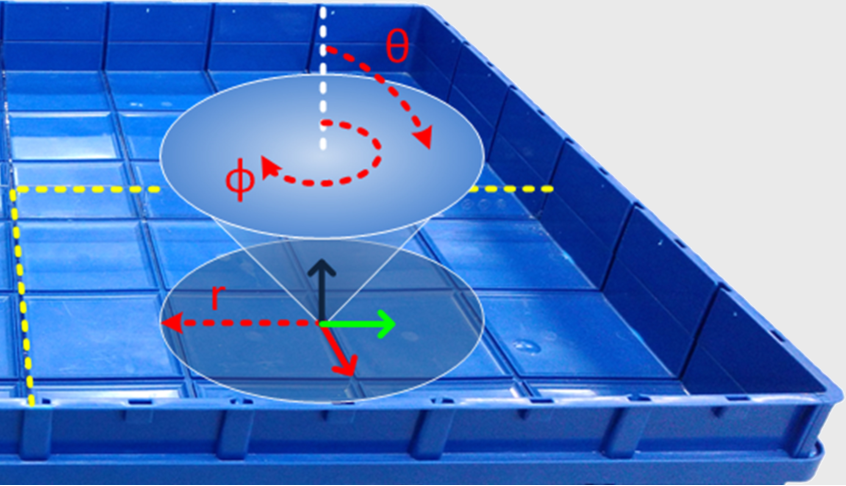
\includegraphics[trim={0cm 0cm 0cm 0cm},clip,width=1\linewidth,angle=0]{Cap4/Figuras/workspace_filter2_gray_bg.pdf}}
\end{tcolorbox}
\caption{Workspace filter 3D representation.}
\label{fig:workspace_filter_3d_representation}
}%end resizebox
\end{figure}

The pipeline descriptor is presented in Snippet \ref{code:workspace_filter}. The first parameter to definition is the ``$ws$\_$base$\_$frame$'' which is the frame name that defines the sphere origin with Z-axis as the reference to angles limits. Thus, the threshold boundary limits can be set by the $min\_azimuth\_threshold \quad \phi_{min}$, $max\_azimuth\_threshold \quad \phi_{max}$, $min\_polar\_threshold \quad \phi_{min}$, $min\_radius\_threshold \quad \phi_{max}$, $min\_radius\_threshold \quad \phi_{max}$ parameters. The angles limits can be defined within a range from -180 to 180 degrees and length from 0 to $\infty$ meters. Any candidate, or associated approach vector, that extrapolate these boundaries are excluded. In the ``$plot\_ws$'' parameter enables workspace 3D visualisation. It is useful to debug and calibrate but it is unnecessary to perform the grasping task.


% and its parameters is described below:

%\begin{itemize_jp}
%    \item \textbf{ws$\_$base$\_$frame:} frame that define the sphere origin. Z-axis is the reference to angles limits.
%    \item \textbf{min$\_$azimuth$\_$threshold $\phi_{min}$:} minimum azimuth angle (from -180 to 180 degrees);
%    \item \textbf{max$\_$azimuth$\_$threshold $\phi_{min}$:} maximum azimuth angle (from -180 to 180 degrees);
%    \item \textbf{min$\_$polar$\_$threshold $\Theta_{min}$:} minimum polar angle (from -180 to 180 degrees);
%    \item \textbf{max$\_$polar$\_$threshold $\Theta_{max}$:} maximum polar angle (from -180 to 180 degrees);
%    \item \textbf{min$\_$radius$\_$threshold $r_{min}$:} minimum radius length (from 0 to +inf meters);
%    \item \textbf{max$\_$radius$\_$threshold $r_{max}$:} maximum radius length (from 0 to +inf meters);
%    \item \textbf{plot$\_$ws:} tag to enable workspace 3D visualisation. It is useful to debug and calibration but it is unnecessary to perform the grasping task.
%\end{itemize_jp}


%\begin{minipage}{1\textwidth} 
\begin{snippet}[h!]
\centering
\resizebox{0.75\textwidth}{!}{%
	\begin{tcolorbox}
 \lstinputlisting[%caption= Workspace filter pipeline descriptor example.,
                  abovecaptionskip=3pt,
                  captionpos=b,
                  style=yaml,
                  linerange={0-10},
                  firstnumber=25,
                  %label=code:workspace_filter
                  ]
                  {Cap4/codes/workspace_filter_heuristic.yaml}
\end{tcolorbox}
}
\caption{Workspace filter pipeline descriptor example.}
\label{code:workspace_filter}
\end{snippet}
%\end{minipage}


\subsection{Collision Filter}
\label{cap4:modular_grasping_architecture:sec:grasp_selection:subsec:collision_filter}

The collision filter is a method that discard candidates that cause collision between the gripper's finger and the scene (or other objects). The fingers trajectory is considered, i.e., the trajectory from open pose to close gripper's finger. The point cloud of the scene must be provided and the collision shape volume must be defined. The Figure~\ref{fig:collision_filter_3d_representation} shows an example of a collision volume (i.e. two collision boxes) defined in 3D representation.


\begin{figure}[h!] %because of cas-sc
\resizebox{0.8\textwidth}{!}{%
\begin{tcolorbox}
% \centerline{\includegraphics[trim={7cm 8cm 7cm 9cm},clip,width=1\linewidth,angle=0]{Cap2/Figuras/friction_contact.pdf}}
\centerline{\includegraphics[trim={0cm 0cm 0cm 0cm},clip,width=1\linewidth,angle=0]{Cap4/Figuras/collision_box_gray_bg.pdf}}
\end{tcolorbox}
\caption{Collision filter 3D representation. The blue boxes define the collision volume.}
\label{fig:collision_filter_3d_representation}
}%end resizebox
\end{figure}

The pipeline descriptor is presented in Snippet \ref{code:workspace_filter}. The input scene cloud to check for collision is defined by ``$cloud$\_$topic$'' while the number of acceptable collision points between the scene point cloud and the collision volume is performed by ``$collision$\_$threshold$'' parameter. It is also possible to reduce the scene input cloud by applying a voxel grid model. By this, the boolean parameters ``$voxel$\_$grid$\_$filter/activate$'' should be set with its tridimensional ``$voxel$\_$grid$\_$filter/leaf$\_$size$'' array. Regarding the finger collision, it is necessary to define  collisions' shapes/volume definition such as pose and dimension. The ``$collisions/show\_shapes$'' it is a parameter tag to enable collision shapes 3D visualisation. It is useful to debug and calibration but it is unnecessary to perform the grasping task.

% and its parameters is described below:


%``$$''

%\begin{itemize_jp}
%    \item \textbf{cloud$\_$topic:} input scene cloud to check for collision;
%    \item \textbf{collision$\_$threshold:} the number of acceptable collision points between the scene point cloud and the collision volume;
%    \item \textbf{voxel$\_$grid$\_$filter/activate:} activate or not a down-sample voxel grid filter into input scene;
%     \item \textbf{voxel$\_$grid$\_$filter/leaf$\_$size:} voxel's grid leaf size;
%    \item \textbf{collisions/gripper$\_$tcp$\_$frame}  gripper tcp frame id used to define the shape/volume. The TCP must be closed;
%    \item \textbf{collisions/show$\_$shapes} tag to enable collision shapes 3D visualisation. It is useful to debug and calibration but it is unnecessary to perform the grasping task.
%    \item \textbf{shapes:} collisions' shapes/volume definition such as pose and dimension.
%
%\end{itemize_jp}

%\begin{minipage}{1\textwidth} 
\begin{snippet}[h!]
\centering
\resizebox{0.75\textwidth}{!}{%
	\begin{tcolorbox}
 \lstinputlisting[%caption= Collision filter pipeline descriptor example.,
                  abovecaptionskip=3pt,
                  captionpos=b,
                  style=yaml,
                  linerange={0-38},
                  firstnumber=25,
                  %label=code:collision_filter
                  ]
                  {Cap4/codes/collision_filter.yaml}
\end{tcolorbox}
}
\caption{Collision filter pipeline descriptor example.}
\label{code:collision_filter}
\end{snippet}
%\end{minipage}


